\chapter{Antenna calculation and simulations}
In this thesis, the chosen transceiver has a operating frequency range from 2400 to 2525MHz, this means that when calculating and simulating the antennas, it is easier to go with a fixed frequency, therefore the center frequency will be used which is 2463MHz or 2463.000.000Hz.

By using the electromagnetic waves function the wavelength can be derived:

\begin{equation}
  f = \frac{c}{\lambda}
\end{equation}

Where f is frequency in Hz, c is the speed of light in meters m/s and $\lambda$ is the wavelength in meters m. 

Wavelength is:

\begin{equation}
  \lambda = \frac{c}{f} \Rightarrow \lambda = \frac{299782458 [m/s]}{2.463.000.000 [Hz]} = 0.1217 meters
\end{equation}

\section{4NEC2}
As explained in the introduction, the 4NEC2 program is made by a radio amateur named Arie Voors\cite{4nec2}, with the goal of being a open source program to help other radio amateurs simulate antennas. This program is not the best of all programs, but as a open source tool and for what is needed in this thesis it will do the job. Some of the things that the program can do is: near and far field analysis, showing VSWR, gain, impedance, half-power beam width and antenna efficiency. The program can also analyze an antenna in different situation, such as: free-space, perfect ground and real ground. It can show a 3-dimensional picture of the radiation pattern for the antenna, but it can also plot the radiation pattern in 2-dimension, for the vertical an horizontal plane, as seen in figure 2.19 and 2.20. furthermore, it is capable of showing a smith chart and impedance matching an antenna to any given impedance, using either an L-filter, Pi-network or T-network. The program can also optimize an antenna, buy changing a given variable, it could be the length of a specific wire, to aim for a higher gain or better VSWR. The downside of this program, is that it is hard to draw complex structures, such as a folded dipole or anything that is circular. Furthermore this the program can not simulate patch antennas, see section 2.6.6 \textit{Microstrip patch antenna}. It is not within the scope of this thesis to explain how to use the program, there are tutorials on the internet that explains how to use the program, moreover, there is a guide on the original website on how to use the program, see reference\cite{4NEC2Guide}. 

\begin{figure}[h!]
\centering
%\hspace*{-2.3cm}
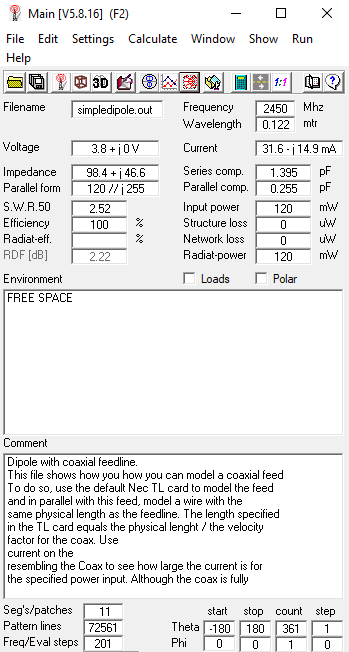
\includegraphics[scale=0.60]{figures/4nec2.PNG}
\caption{Showing the front page of the 4NEC2 program}
\end{figure}

\newpage

\section{Yagi calculator}
The Yagi calculator is also an open source program made by a radio amateur, John Drew\cite{yagical}, with the goal of making it easier to quickly design and build a yagi antenna. This program does not simulate the antenna, but rather uses a template made by years of experimentation in the radio amateur world, even the front page of the program states that, see figure 3.2. The program is capable of calculating the size of the yagi-uda elements, the dimension of the driven element (folded dipole) and the distance between each elements, see section 2.6.7 \textit{Yagi-uda and cross-yagi-uda antennas}. It can calculate the half-power beam width, the gain for each director added. If a coaxial cable is specified the program can calculate the length of the matching stub, to match the yagi antenna to an impedance of $50\Omega$.

\begin{figure}[h!]
\centering
%\hspace*{-2.3cm}
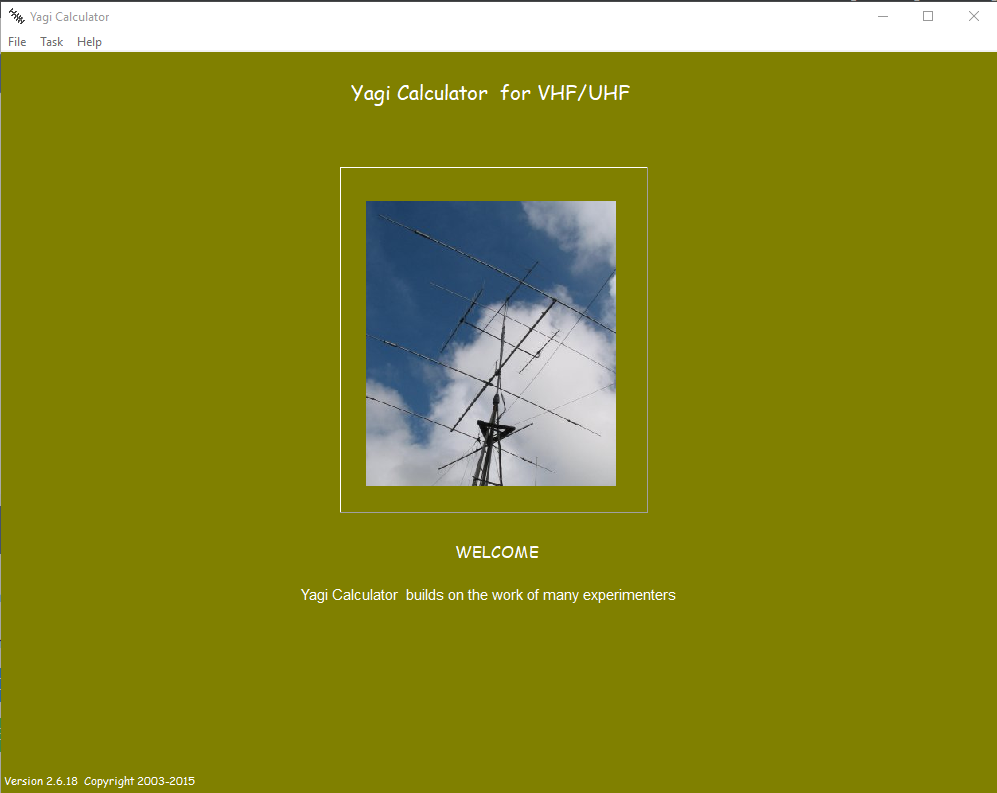
\includegraphics[scale=0.5]{figures/YagiCalculator.PNG}
\caption{Showing the front page of the Yagi calculator program}
\end{figure}

\newpage

\section{Half-wave dipole}
The length of a half-wave dipole, is as the name stated the half of the used wave. Above the wavelength for the center frequency is calculated to be $0.1224meters$, thus the total length of a half-wave dipole is:

\begin{equation}
  Dipole_L = \frac{\lambda}{2} = 0.0609 meters
\end{equation}

Each side elements on the dipole has a length of:

\begin{equation}
  Dipole_E = \frac{\lambda}{4} = 0.0304 meters
\end{equation}

The above result is used in the 4NEC2 program to simulate the antenna, the result from the simulation in free-space (meaning no ground effects) is: 

\begin{figure}[h!]
\centering
%\hspace*{-2.3cm}
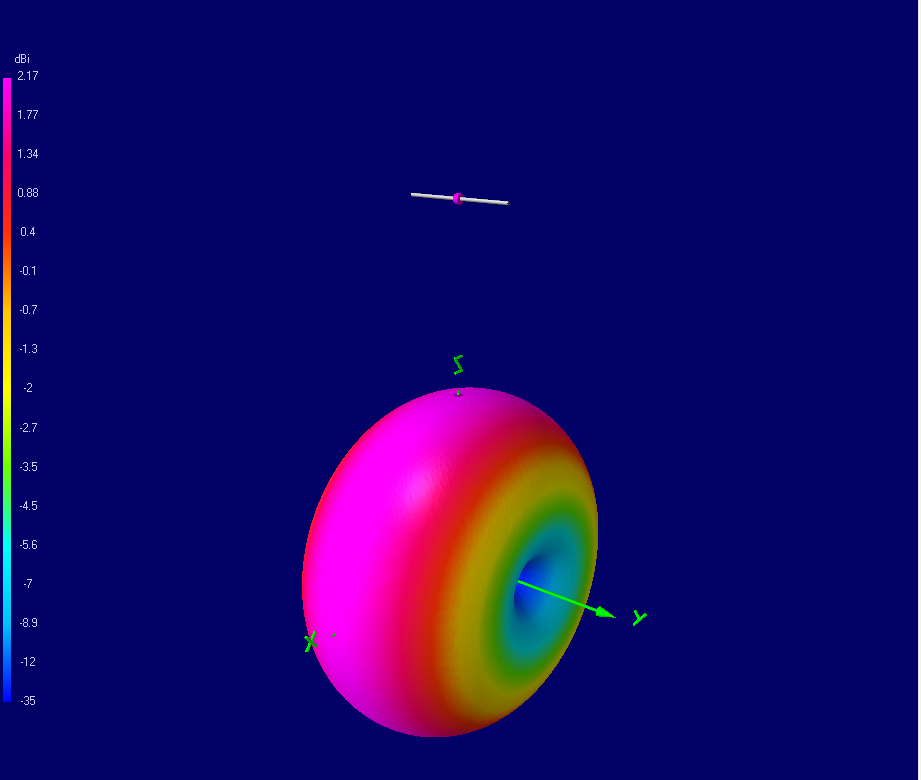
\includegraphics[scale=0.5]{figures/SimulatedDipoleRad.PNG}
\caption{Half-wave dipole antenna 3-dimensional radiation pattern and gain}
\end{figure}

\begin{figure}[h!]
\centering
%\hspace*{-2.3cm}
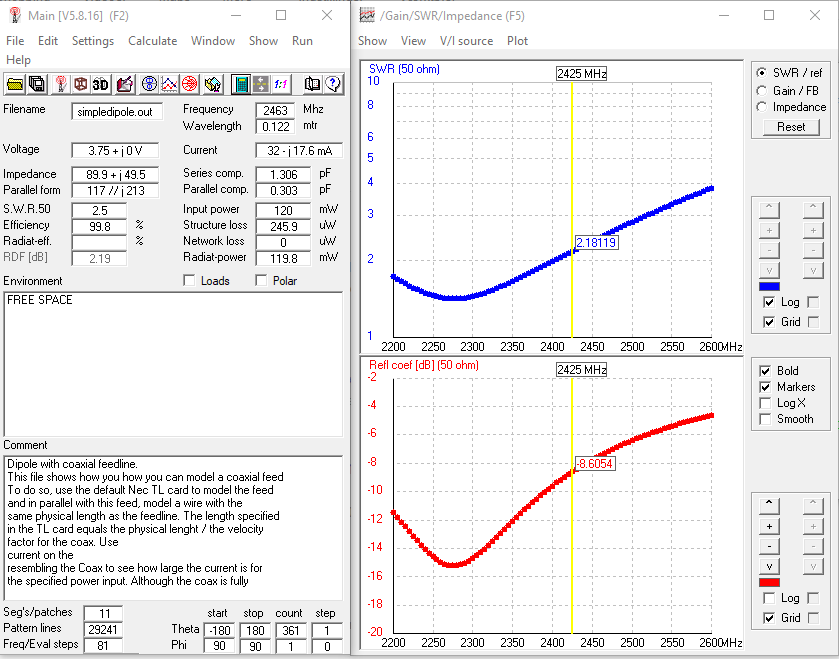
\includegraphics[scale=0.5]{figures/DipoleImpedanceVSWR.PNG}
\caption{Half-wave dipole antenna radiation Impedance and VSWR}
\end{figure}

\begin{figure}[h!]
\centering
%\hspace*{-2.3cm}
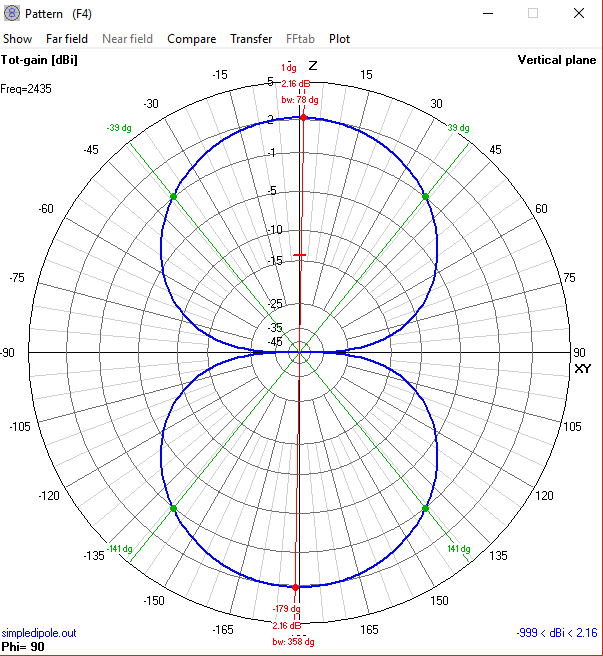
\includegraphics[scale=0.5]{figures/DipoleRadiationPattern.PNG}
\caption{Half-wave dipole antenna 2-dimensional radiation pattern}
\end{figure}

\section{Sleeved dipole}
The sleeved dipole was simulated by reverse engineering a sleeved dipole bought from china, s. 




\section{Quaterwave monopol}
%length of Quaterwave monopol each arm
% show the simulations and results
\section{Helical}
%use the matlab code in conjunction with the theory part

\section{Yagi-uda and cross yagi-uda}
%% use yagi antena software and merge it with repport about cross-yagi antenna, DONT SIMULATE IT, since you are not using this type of antenna. 

\section{Partial conclusion}